\documentclass[12pt]{article}

\usepackage[utf8]{inputenc}
\usepackage{latexsym,amsfonts,amssymb,amsthm,amsmath}
\usepackage{graphicx}
\usepackage{titling}
\usepackage{gensymb}

\setlength{\parindent}{0in}
\setlength{\oddsidemargin}{0in}
\setlength{\textwidth}{6.5in}
\setlength{\textheight}{8.8in}
\setlength{\topmargin}{0in}
\setlength{\headheight}{18pt}
\setlength{\headsep}{-30pt}
\newcommand{\overbar}[1]{\mkern 1.5mu\overline{\mkern-1.5mu#1\mkern-1.5mu}\mkern 1.5mu}
\author{Bryan Wang}

\setlength{\droptitle}{-4em}
\title{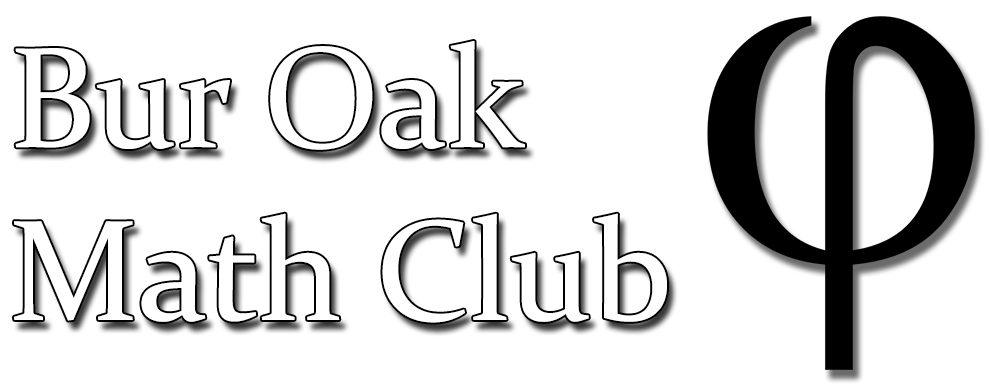
\includegraphics[width=10cm]{Bur Oak Math Club Banner Bold.png}\\\vspace{0.25in} Gr.11-12 Class 1 Homework (Triangles)}

\begin{document}
\maketitle

\subsection*{Exercise 1}
How many ways can we form a non-degenerate triangle by choosing three distinct numbers from the set \{1, 2, 3, 4, 5\} as the sides.
\vspace{1.5in} %Leave space for comments!

\subsection*{Exercise 2}
In the given figure, $\overbar{DB}$ bisects the exterior angle $\angle$EBA of $\Delta$ABC. If $\overbar{AB}$ = 6, $\overbar{BC}$ = 10, and $\overbar{AC}$ = 12, find $\overbar{DA}$.
\begin{figure}[htp]
    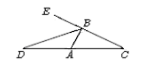
\includegraphics[width=6cm]{img1.png}
\end{figure}
\vspace{1in} %Leave more space for comments!

\subsection*{Exercise 3}
Triangle $\Delta$ABC has a right angle at B. Point D is the foot of the altitude from B, $\overbar{AD}$ = 3, and $\overbar{DC}$ = 4. What is the area of $\Delta$ABC? (AMC 10).
\begin{figure}[htp]
    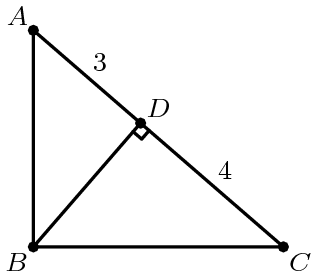
\includegraphics[width=5cm]{img3.png}
\end{figure}
\vspace{1.5in}

\subsection*{Exercise 4}
Triangle $\Delta$AMC is isosceles with  $\overbar{AM}$ =  $\overbar{AC}$. Medians $\overbar{MV}$ and $\overbar{CU}$ are perpendicular to each other, and $\overbar{MV}$ = $\overbar{CU}$ = 12. What is the area of $\Delta$AMC? (AMC 10).
\begin{figure}[htp]
    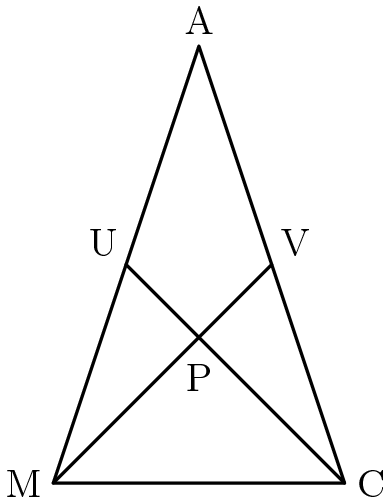
\includegraphics[width=4cm]{img2.png}
\end{figure}
\vspace{2in}

\subsection*{Exercise 5}
Inside the right triangle $\Delta$ABC (angle C is the right angle) a point O is chosen so that $\Delta$OAB, $\Delta$OBC, $\Delta$OAC have the same area. Find the length of $\overbar{OC}$ if $\overbar{AB}$ = 51.
\vspace{3in}

\subsection*{Exercise 6}
Triangle $\Delta$ABC is isosceles with $\overbar{AC}$ = $\overbar{BC}$ and $\angle$ACB = 106$\degree$. Point M is the interior of the triangle so that $\angle$MAC = 7$\degree$ and $\angle$MCA = 23$\degree$. Find the number of degrees in $\angle$CMB. (AIME).
\begin{figure}[htp]
    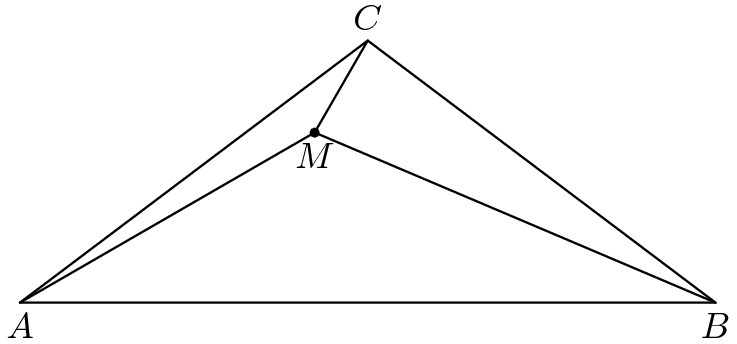
\includegraphics[width=8cm]{img4.png}
\end{figure}
\vspace{2in}


\end{document}
